%----------------------------------------------------------------------------------------
%	PACKAGES AND OTHER DOCUMENT CONFIGURATIONS
%----------------------------------------------------------------------------------------

\documentclass{article}

\usepackage{fancyhdr} % Required for custom headers
\usepackage{lastpage} % Required to determine the last page for the footer
\usepackage{extramarks} % Required for headers and footers
\usepackage[usenames,dvipsnames]{color} % Required for custom colors
\usepackage{graphicx} % Required to insert images
\usepackage{listings} % Required for insertion of code
\usepackage{courier} % Required for the courier font
\usepackage{lipsum} % Used for inserting dummy 'Lorem ipsum' text into the template
\usepackage{parskip}
% Margins
\topmargin=-0.45in
\evensidemargin=0in
\oddsidemargin=0in
\textwidth=6.5in
\textheight=9.0in
\headsep=0.25in

\linespread{1.1} % Line spacing

% Set up the header and footer
\pagestyle{fancy}
\chead{} % Top left header
\lhead{\hmwkClass\  \hmwkTitle} % Top center head
\rhead{} % Top right header
\lfoot{\lastxmark} % Bottom left footer
\cfoot{} % Bottom center footer
\rfoot{Page\ \thepage\ of\ \protect\pageref{LastPage}} % Bottom right footer
\renewcommand\headrulewidth{0.4pt} % Size of the header rule
\renewcommand\footrulewidth{0.4pt} % Size of the footer rule

\setlength\parindent{0pt} % Removes all indentation from paragraphs

%----------------------------------------------------------------------------------------
%	CODE INCLUSION CONFIGURATION
%----------------------------------------------------------------------------------------

% \definecolor{MyDarkGreen}{rgb}{0.0,0.4,0.0} % This is the color used for comments
\lstloadlanguages{C} % Load C syntax for listings, for a list of other languages supported see: ftp://ftp.tex.ac.uk/tex-archive/macros/latex/contrib/listings/listings.pdf
\lstset{language=C,frame=single,keywordstyle=[1]\color{Blue}\bf} % Use C in this example      



\newcommand{\csnippet}[2]{
\begin{itemize}
\item[]\lstinputlisting[caption=#2,label=#1]{#1.c}
\end{itemize}
}

%----------------------------------------------------------------------------------------
%	DOCUMENT STRUCTURE COMMANDS
%----------------------------------------------------------------------------------------

% Header and footer for when a page split occurs within a problem environment
\newcommand{\enterProblemHeader}[1]{
\nobreak\extramarks{#1}{#1 continued on next page\ldots}\nobreak
\nobreak\extramarks{#1 (continued)}{#1 continued on next page\ldots}\nobreak
}

% Header and footer for when a page split occurs between problem environments
\newcommand{\exitProblemHeader}[1]{
\nobreak\extramarks{#1 (continued)}{#1 continued on next page\ldots}\nobreak
\nobreak\extramarks{#1}{}\nobreak
}

\setcounter{secnumdepth}{0} % Removes default section numbers
\newcounter{homeworkProblemCounter} % Creates a counter to keep track of the number of problems

\newcommand{\homeworkProblemName}{}
\newenvironment{homeworkProblem}[1][Problem \arabic{homeworkProblemCounter}]{ % Makes a new environment called homeworkProblem which takes 1 argument (custom name) but the default is "Problem #"
\stepcounter{homeworkProblemCounter} % Increase counter for number of problems
\renewcommand{\homeworkProblemName}{#1} % Assign \homeworkProblemName the name of the problem
\section{\homeworkProblemName} % Make a section in the document with the custom problem count
\enterProblemHeader{\homeworkProblemName} % Header and footer within the environment
}{
\exitProblemHeader{\homeworkProblemName} % Header and footer after the environment
}

\newcommand{\problemAnswer}[1]{ % Defines the problem answer command with the content as the only argument
\noindent\framebox[\columnwidth][c]{\begin{minipage}{0.98\columnwidth}#1\end{minipage}} % Makes the box around the problem answer and puts the content inside
}

\newcommand{\homeworkSectionName}{}
\newenvironment{homeworkSection}[1]{ % New environment for sections within homework problems, takes 1 argument - the name of the section
\renewcommand{\homeworkSectionName}{#1} % Assign \homeworkSectionName to the name of the section from the environment argument
\subsection{\homeworkSectionName} % Make a subsection with the custom name of the subsection
\enterProblemHeader{\homeworkProblemName\ [\homeworkSectionName]} % Header and footer within the environment
}{
\enterProblemHeader{\homeworkProblemName} % Header and footer after the environment
}

%----------------------------------------------------------------------------------------
%	NAME AND CLASS SECTION
%----------------------------------------------------------------------------------------

\newcommand{\hmwkTitle}{Assignment\ \#1} % assignment title
\newcommand{\hmwkDueDate}{Monday,\ November\ 3,\ 2014} % due date
\newcommand{\hmwkClass}{Programming Concurrent Systems} % class
\newcommand{\hmwkClassTime}{} % lecture time
\newcommand{\hmwkClassInstructor}{} % lecturer
\newcommand{\hmwkAuthorName}{Alyssa - Ilias} %name

%----------------------------------------------------------------------------------------
%	TITLE PAGE
%----------------------------------------------------------------------------------------

\title{
\vspace{2in}
\textmd{\textbf{\hmwkClass:\ \hmwkTitle}}\\
\normalsize\vspace{0.1in}\small{Due\ on\ \hmwkDueDate}\\
\vspace{0.1in}\large{\textit{\hmwkClassInstructor\ \hmwkClassTime}}
\vspace{3in}
}

\author{\textbf{\hmwkAuthorName}}


%----------------------------------------------------------------------------------------

\begin{document}

\maketitle

%----------------------------------------------------------------------------------------
%	TABLE OF CONTENTS
%----------------------------------------------------------------------------------------

%\setcounter{tocdepth}{1} % Uncomment this line if you don't want subsections listed in the ToC

\newpage
\tableofcontents
\newpage

%----------------------------------------------------------------------------------------
%	Introduction
%----------------------------------------------------------------------------------------
\begin{homeworkProblem}[Introduction]
For this assignment, we were asked to implement a simulation of heat dissipation on the surface of a cylinder.
The implementation is sequential, and will serve as a basis for the following assignments where we will provide a parallelized solution.
\\\\
The surface is represented as a N x M matrix, where each matrix element/cell represents the temperature value.
There is another identicallly-sized matrix containing the per-cell conductivity, with values in the range [0,1].
Depending on the conductivity of each point and its 8 surrounding neighbours, a new temperature is computed, in an iterative manner.
Specifically, the following formula describes the computations used for the simulation:
\\\\
\(t' = c_t*t + (1-c_t) * \frac{\sqrt{2}}{\sqrt{2}+1} * \frac{1}{4} * \sum_{i=1}^{4} a_i 
    + (1-c_t) * \frac{1}{\sqrt{2}+1} * \frac{1}{4} * \sum_{j=1}^{4} b_j \) , where 
\\\\
\(t'\) is the new temprature value \\
\(t\)  is the point's temprature value \\
\(c_t\) is the point's respective conductivity \\
\(a_i\) are the direct neighbour temperature values \\
\(b_j\) are the diagonal neighbour temperature values
\\\\
The M columns of the matrix represent the cyclic dimension of the cylinder; note that the first and last columns are neighbours.
The other dimension has a fixed boundary on the first and last rows; the neighbours of the boundary, not represented in our matrices,
have a fixed temperature equal to the initial temprature value of these boundary cells.
\end{homeworkProblem}
%----------------------------------------------------------------------------------------
%	Solution Description
%----------------------------------------------------------------------------------------

% To have just one problem per page, simply put a \clearpage after each problem

\begin{homeworkProblem}[Solution Description]
In our solution we use two matrices, \textbf{t\_prev} and \textbf{t\_next}, dynamically allocated and stored in pointers.
The matrix \textbf{t\_prev} contains the temperature values from the previous iteration, initially the start temperatures.
In an iterative process, we compute a new value for every point, as depicted by Listing 1, and we store these values in \textbf{t\_next}.
When all points have been (re)computed, we swap the pointers.

The iterative process ends when the maximum temperature difference is less than a user-provided threshold,
or the number of iterations have reached a user provided maximum.

These matrices allocated as one large block (for efficiency) and are stored in row-major order; we iterate over them
row-by-row, since the input is stored in this way, and going column-by-column would lead to a large number of cache
lines being required and a reduction in performance due to this.

\csnippet{main_calculation}{Snippet of the main calculation}

During the iterations, we gather information on the heat dissipation process.
This information is computed periodically, depending on the user-provided configuration.
Although this is not a parallelised solution, we describe this here as a reduction step, since
the operations (finding minimum/maximum values and calculating the average) are ones which we
will have to perform as a reduction. \\
In this step, we calculate (among other things) the maximum temperature difference.
It is important that we do this reduction step periodically, in order to effectively stop iterating
in the case the difference is less than the threshold, but the reduction step also causes unnecessary overhead.
\\\\
We currently perform the reduction step separately from the calculation, which avoids the branches appearing
in the main loops.
\\\\
The wraparound (left/right) and boundaries (top/bottom) also add some complexity. Our initial approach for the
wraparound (checking for the left/right sides explicitly in the inner loop) led to branches in the inner loop
causing performance problems, so we refactored the calculation code into an (inlined) function, and call it
for the first/last columns explicitly before/after the inner loop. We also attempted to use a modulo calculation,
but this resulted in worse performance (and increasing the column size of the matrix so that we could do this
with an AND operation instead seemed unnecessarily wasteful, so we didn't even try that).

\csnippet{inner_loop}{Innermost loop handling first/last columns separately}

The top/bottom boundaries could be handled by allocating two extra rows in the matrices and copying the initial
values into these rows, but instead we simply explicitly check for these cases in the outer loop and use
pointers to the initial temperature values for the \texttt{rowup} or \texttt{rowdown} pointers as needed.

\csnippet{boundary_checks}{The explicit checks for the boundary rows.}

We also tried precalculating all the direct/diagonal neighbour weights, so that we could simply multiply these
with the sum of the relevant cell values (you can see this in the supplied code in the sections marked \texttt{PRECALC\_CND}),
but this not only increased the RAM requirements dramatically, but also resulted in worse performance.
\\\\
Instead, we store the weight multipliers as constants in the source code, which resulted in a slight performance improvement,
but this might not be justified in all circumstances given the reduction in clarity of the code.

\csnippet{constants}{Weight multiplier constants}

Our extensive use of pointer arithmetic/etc in the code could be argued to be worse for maintainability, and makes it more
difficult to use e.g., C99-style multi-dimensional virtual arrays, but also makes it clearer what is happening in the resulting code. 
\\\\
Tweaking compiler flags appeared unproductive; the ancient gcc 4.4 on the DAS 4 head nodes doesn't support
\texttt{-march=westmere}, but \texttt{-march=core2} didn't significantly help performance. Trying flags like
\texttt{-O3} and \texttt{-funroll-loops} resulted in significantly worse performance. The lack of access to
useful profiling tools on the DAS 4 nodes was also a problem. For future work it might be preferable to replicate
the compilation environment elsewhere, but the lack of an OpenACC compiler makes this problematic, since the framework requires one be present. We also didn't see any performance improvements from trying to use the \texttt{restrict} keyword.
\end{homeworkProblem}

%----------------------------------------------------------------------------------------
%	Evaluation
%----------------------------------------------------------------------------------------

\begin{homeworkProblem}[Evaluation]
%\lipsum[2]
For the evaluation of our code we run a set of experiments. Following are the outcome observations:
\\\\
From the following graph we can see that if we do the reduction step on every iteration the impact is performance drawback. But we see that if we report periodically - even often - the overhead is little and the convergence is computed as well. This allows the exit condition to be tested more often without an important performance issue.
\\\\
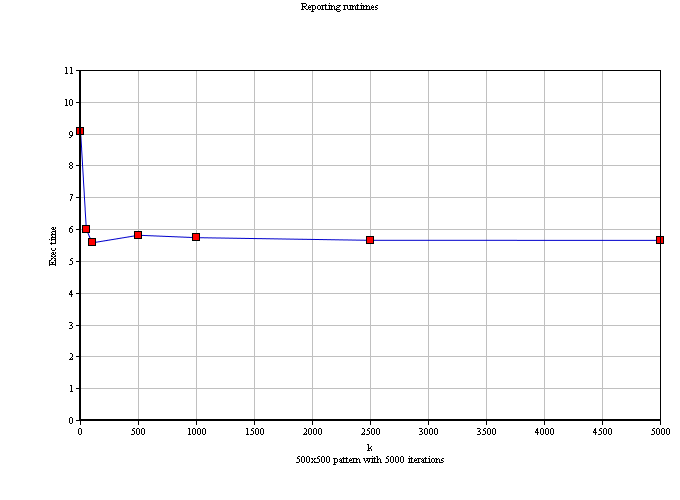
\includegraphics[width=0.75\columnwidth]{kshow.png}
\\\\
The following figure depicts wall time as opposed to element number. As expected the more elements, the more execution time in a linear relation. This experiment will serve for a latter comparison with parallelized implementation.
\\\\
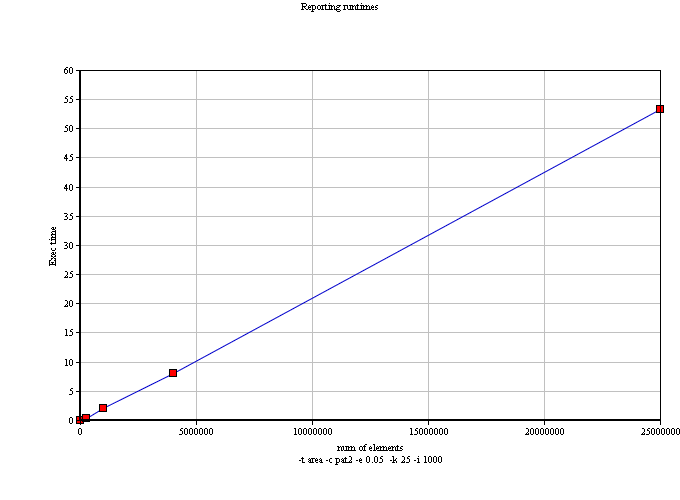
\includegraphics[width=0.75\columnwidth]{walltime.png}
\clearpage
Moreover, we collected some results before and after the optimizations to remove the branches from the inner loop:\\\\
heat -t plasma\_1000x1000.pgm -c pat2\_1000x1000.pgm -m 1000 -n 1000 -e 0.1 -k 1 -i 20 \\
Execution time before: 0.268016 \\
Execution time after: 0.181496 \\
\\\\
heat -t plasma\_1000x1000.pgm -c pat2\_1000x1000.pgm -m 1000 -n 1000 -e 0.1 -k 20 -i 20  \\
Execution time before: 0.173204 \\
Execution time after: 0.138695 \\
\\\\
heat -t plasma\_1000x1000.pgm -c pat2\_1000x1000.pgm -m 1000 -n 1000 -e 0.0 -k 100000 -i 5000 \\
Execution time before: 40.801666 \\
Execution time after: 26.257804 \\
\\
We can see a big performance improvement from the optimization discussed in our solution.
\\\\
In this experiment we compared different widths and heights keeping the same amount of elements for us to see if the boundary affects the performance. We can see that there is a difference between different dimensions. This is logical because we have optimized column traversal.
\\\\
heat -t areas\_100000x10.pgm -c pat2\_100000x10.pgm -m 10 -n 100000 -e 0.0 -k 5000 -i 5000 \\
Execution time: 30.185160 \\
\\\\
heat -t areas\_10x100000.pgm -c pat2\_10x100000.pgm -m 100000 -n 10 -e 0.0 -k 5000 -i 5000 \\
Execution time: 26.802325 \\
\\\\
heat -t areas\_1000x1000.pgm -c pat2\_1000x1000.pgm -m 1000 -n 1000 -e 0.0 -k 5000 -i 5000 \\
Execution time: 27.313954 \\
\\\\
For our last experiment we made observations about FLOP/s. Generally the more FLOP/s the more efficient is the implementation since at the end there should be the same amount of floating point instructions that were executed.  
\\\\
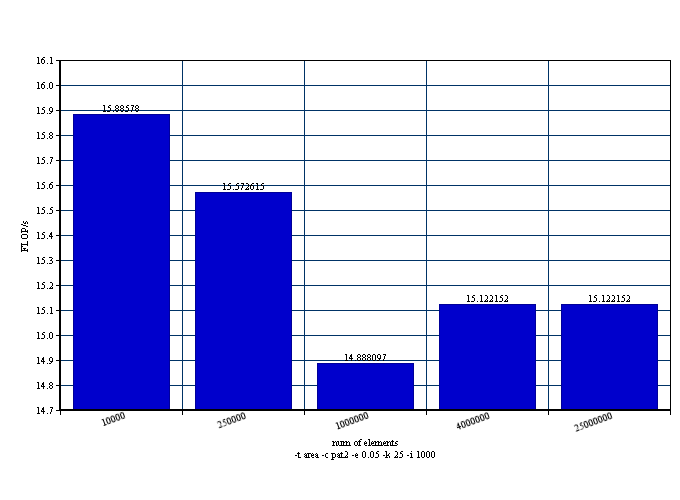
\includegraphics[width=0.75\columnwidth]{flops.png}
\\\\
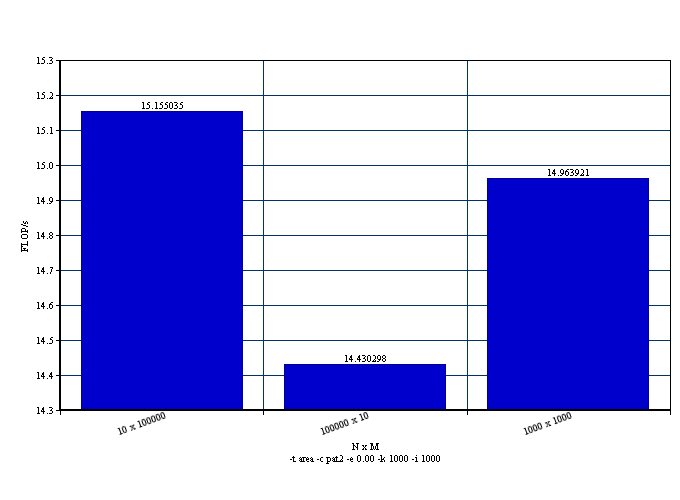
\includegraphics[width=0.75\columnwidth]{flops2.png}
\\\\
Note that the presented times are the time from the first call to main, up to and including the final
run through the loop. You can exclude the final loop from the calculations when terminating due to
exceeding the iteration count by adding an \texttt{if (!done)} before the assignment to \texttt{r->time}.

\end{homeworkProblem}

%----------------------------------------------------------------------------------------

\end{document}
